\section{Descripción del Problema}\label{descripciuxf3n-del-problema}

Se considerá una empresa dedicada a la venta y renta de inmuebles, cuyos canales  de venta són  entrevistas y  llamadas telefónicas. Ha decidido invertir en un sitio web donde publica el listado de propiedades a ofertar. Como en la mayoria de sitios web, el diseño se centra únicamente en un portal informativo. Con frecuencia buscando llamar la atención del usuario utilizando elementos dinámicos basados en imágenes o videos,  de tal manera que no es posible identificar información relevante o es imposible realizar una búsqueda en texto para localizar un artículo especifico. Por consecuencia los clientes que visitan el sitio (ver info de visitas) observan que resulta muy complicado localizar alguna propiedad relevante, o simplemente toma demasiado tiempo navegar pagina a página para encontrar lo que se requiere. 

Este ejemplo es el caso de la mayoria de negocios mexicanos que utilizan un portal web para anunciarse y no aprovechan la interacción con sus clientes.
Dentro de la ciudad de Morelia, se han detectado poco más de 30 inmobiliarias que utilizan portales para promoción, incluso las principales constructoras (Arko, Habicasa) utilizan  portales de tipo informativo. Muy pocos son los que realizan alguna encuentas o registro para conocer a sus clientes. Por lo que este proyecto busca incrementar la cantidad de información que un usuario promedio recibe al consultar una propiedad. Para ello se incluyen sugerencias de propiedades similares con el fin de mantener al usuario más tiempo en el sitio y por consecuencia incrementar la utilidad de la información. Adicionalmente para mejorar las recomendaciones, durante la navegación se buscará conocer las preferencias del usuario utilizando  breves cuestionarios sobre la información que se está consultando para identificar potenciales opciones. 

\subsection{Metodología}

Nuestra propuesta de diseño se centra en 4 puntos.
\begin{enumerate}
\item Recolección de Datos.
\item Filtrado y Clasificación de los datos.
\item Proporcionar recomendaciones cercanas a las seleccionadas por el usuario.
\item Retroalimentación a través de encuestas de satisfacción al cliente.
\end{enumerate}


\subsection{Recolección de los datos}

Para la recolección, seleccionamos 20 inmobiliarias de la ciudad de Morelia, algunos portales no presentaban listados accesibles y se descartaros.
Del conjunto del que era posible consultar propiedades a traves de una url directa se decidió  utilizar un crawler público{[}6{]} que nos permitiera indexar las paginas web de las inmobiliarias, para obtener una lista de links (ver figura \ref{fig:CrawlerList}), se filtro la lista dejando unicamente las que se refieren a propiedades; almacenando posteriormente los documentos en formato HTML. 
\subsection{Filtrado y Clasificación}

Se extraerá el cuerpo principal de los documento usando el lenguaje de programación python, almacenado cada propiedad en un nuevo conjunto de datos  que convertiremos a un archivo csv para posteriomente  realizar la clasificación de las propiedades. Es importante destacar que para este proyecto no se requiere almacenar en una base de datos relacional la información, debido a que trabajar con texto plano simplifica al análisis y no se requiere interacción por parte del usuario.


\begin{figure}[ht]
\centering
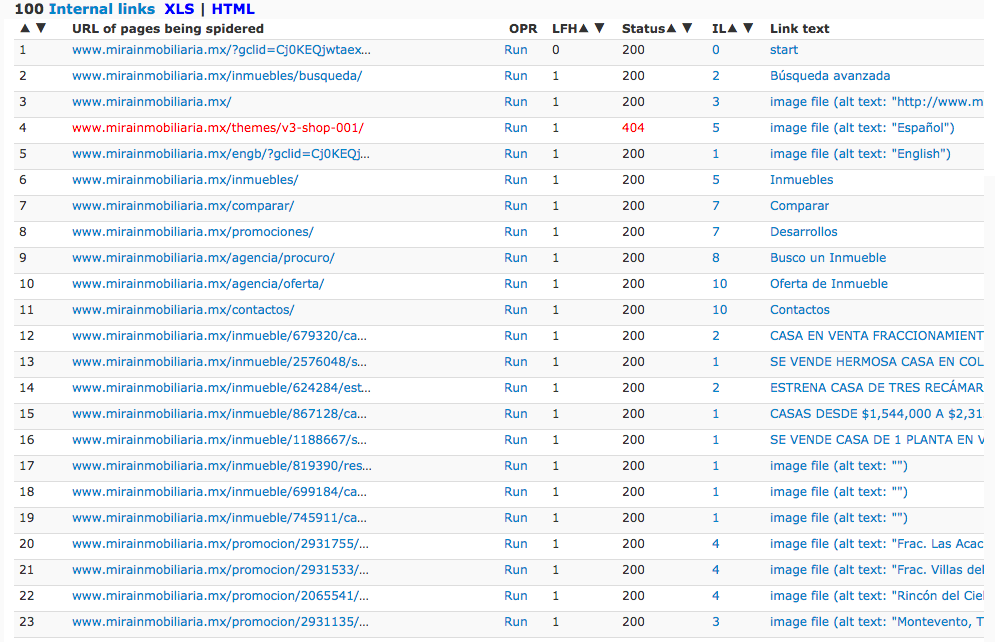
\includegraphics[width=0.8\textwidth]{CrawlerSite.png}
\caption{Listado de Artículos relacionados con propiedades}
\label{fig:CrawlerList}
\end{figure}


\begin{figure}[ht]
\centering
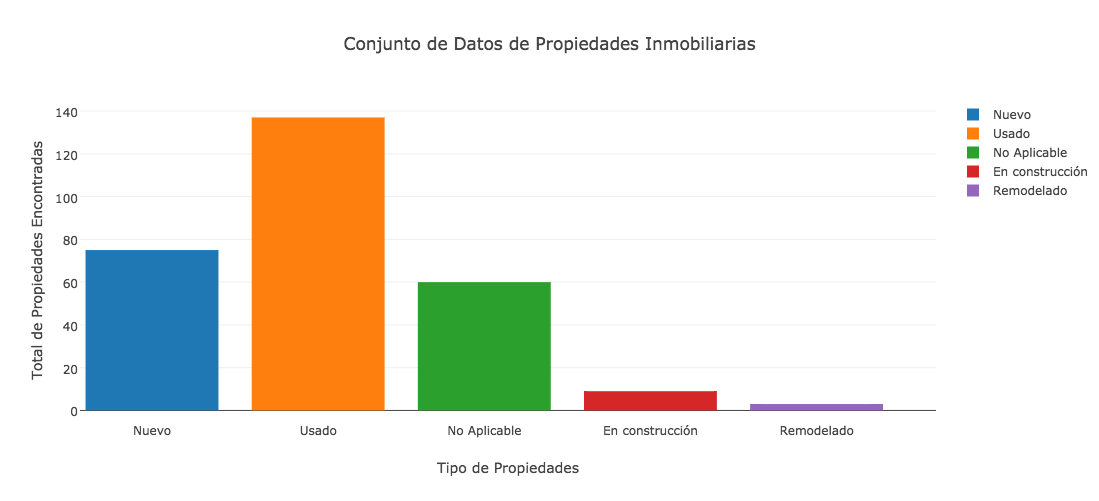
\includegraphics[width=0.8\textwidth]{PropiedadesInmobiliariasEstadoVivienda.png}
\caption{Distribución de Propiedades Tipo de Propiedad}
\label{fig:PropiedadesType}
\end{figure}

\begin{figure}[ht]
\centering
\begin{tabular}{cc}
  \hline
 & Total \\ 
  \hline
Bodega &   5 \\ 
  Casa & 168 \\ 
  Departamento &  24 \\ 
  Edificio &   1 \\ 
  Local &  13 \\ 
  Oficinas &   1 \\ 
  Terreno &  72 \\ 
   \hline
\end{tabular}
\caption{Tabla de Propiedades por Inmueble}
\label{fig:PropiedadesList}
\end{figure}

\subsection{Clasificación de las propiedades}
Para el procesamiento y clasificación de los datos se utilizara el lenguaje de programación R. Las propiedades que descargamos de los portales web se integrarán en un solo listado con aproximadamente 284 registros, las cuales  vienen listadas por Estado de la propiedades (Usado, Nuevo, Construcción), Área construida ($m^2$), Zona (Colonia o barrio de Referencia), Precio, Latitud, Longitud y el tipo de propiedad (ver figura \ref{fig:Dataset}). 


El algoritmo de clasificación es el de vecinos cercanos (KNN), ya que estamos trabajando con variables categóricas. Nuestro objetivo es ofrecer opciones con carácteristicas similares dentro de cada categoria correspondiente.
\begin{figure}[ht]
\centering
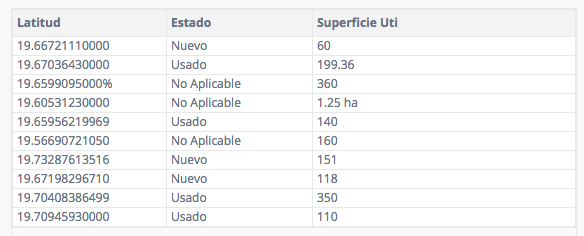
\includegraphics[width=0.8\textwidth]{Dataset.png}
\caption{Dataset de Propiedades Inmobiliarias}
\label{fig:Dataset}
\end{figure}


\subsection{KNN - Nearest Neighbor}
También conocido como (vecino cercano); es el más simple de los algoritmos de aprendizaje máquina que existe y el más utilizado si se trabaja con variables categóricas. Se basa en identificar los k  registros en el conjunto de entrenamiento que son \emph{cercanos} en similaridad. La prueba asigna una clase a la mayoria de los vecinos cercanos similares. El KNN trata las características como coordenadas multidimensionales. Después tomaremos uno o más registros del conjunto de prueba, los cuales serán las selecciones del usuario. 

\subsection{Métrica de similaridad con distancia.}

El KNN requiere una función distancia, o una métrica que mida la similaridad entre dos instancias. El KNN utiliza la distancia euclideana, que es la distancia de un punto con respecto a otro conectados por una línea recta. La distancia euclideana se expresa de la siguiente manera:

\begin{equation}
dist(x,y) = \sqrt{(p_1-q_1)^2 + (p_2-q_2)^2+ \cdots + (p_n - q_n)^2}
\end{equation}

El KNN requiere elegir una cantidad de vecinos cercanos (K) y determinar que tan bien el modelo clasifica nuevos valores. El balance entre sobre ajustar o subajustar el valor de K para el conjunto de entrenamiento es un problema conocido como \textbf{ajuste de la varianza}. En la figura \ref{fig:seleccionK} se observa que si se elige una K muy grande el conjunto se parte dejando algunos puntos clasificados incorrectamente, lo cual se toma como falsos positivos; en cambio si la K se toma muy pequeña se tienen falsos falsos. 
La seleccion de la K se considera en base a la tolerancia de error (la queda a elección  del programador) que se pueda perimitir el clasificador, ajustando así hasta que se encuentra una K entre estos dos extremos.

Cuando se seleccionan los valores de K el impacto de la varianza causa datos ruidosos, los cuales pueden ser incluidos o puede sean ignorados por el sistema.


\begin{figure}[ht]
\centering
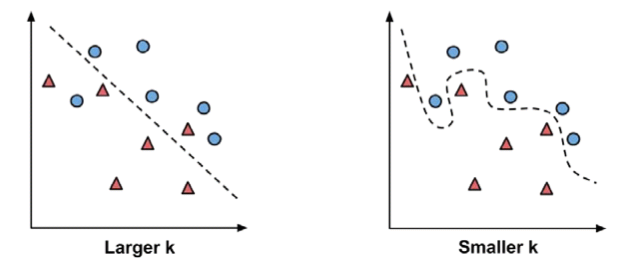
\includegraphics[width=0.5\textwidth]{IMG_0061.png}
\caption{Efectos de seleccionar diferentes valores  de la K en KNN}
\label{fig:seleccionK}
\end{figure}

\begin{figure}[H]
\centering
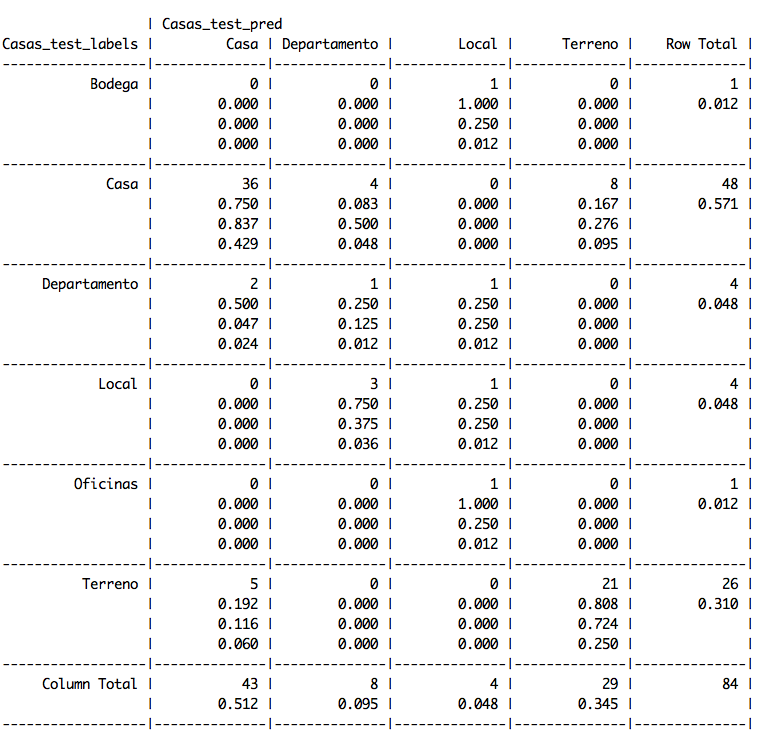
\includegraphics[width=0.8\textwidth]{ModeloPredictivo.png}
\caption{Propiedades recomendadas según la selección del Usuario}
\label{fig:Clasificador}
\end{figure}


\section{Resultados}
A continuación se describe en lenguaje R el algoritmo utilizado para la clasificación utilizando KNN.

\begin{verbatim}

#Clasificador de Casas segun la eleccion
CasasCompletas <- read.csv("DataSet1.csv",header=TRUE)
View(CasasCompletas)
#casasClasificar <- CasasCompletas[,c(1,4,5,7,8,9)]
#View(casasClasificar)
CasasCompletas$Tipo <- factor(CasasCompletas$Inmueble,
             levels=c("Casa","Departamento","Oficinas",
             "Local","Terreno","Bodega"),
             labels=c("Casa","Departamento","Oficinas",
             "Local","Terreno","Bodega"))
CasasCompletas$Estado <- factor(CasasCompletas$Estado,
             levels=c("Nuevo","Usado","No Aplicable",
             "En construccion","Remodelado"), 
             labels=c("Nuevo","Usado","T", "PC","RM"))
CasasCompletas$Oferta <-factor(CasasCompletas$Oferta,
             levels=c("renta","venta"),
             labels=c("renta","venta"))
CasasCompletas$Inmueble <- factor(CasasCompletas$Inmueble,
             levels = c("Casas","Departamento", "Habitacion", 
             "Oficina","Local","Terreno","Edificio"))


round(prop.table(table(CasasCompletas$Estado))*100,digits = 1)

normalizacion <- function(x) {
  return ((x - min(x)) / (max(x) - min(x)))
}

CasasNorm <- as.data.frame(
            lapply(CasasCompletas[c(3,5,6)],normalizacion))

# Clasificacion por KNN

Casas_train <- CasasNorm[1:200,]
Casas_prop <- CasasNorm[201:284,]
Casas_train_labels <- CasasCompletas[1:200,1]
Casas_test_labels <- CasasCompletas[201:284,1]
library('class')
library('gmodels')

Casas_test_pred <- knn(train=Casas_train,test=Casas_prop,
                       cl=Casas_train_labels,k = 6)
Casas_test_pred

# La tabla cruzada nos permite comparar como se clasificaron
# los datos de prueba
CrossTable(x = Casas_test_labels, 
        y = Casas_test_pred, prop.chisq = FALSE)
\end{verbatim}

De la figura ~\ref{fig:Clasificador} las celdas que caen en la diagonal contienen  el numero de registros  donde el KNN encontró propiedades que son similares  con la muestra seleccionada. Se  puede observar que el conjunto de propiedades sugeridas se obtiene al seleccionar  una K  con valor de 6, basándonos en que tenemos 6 posibles clases distintas. Probamos distintos valores de K para refinar la consulta. Al implementar este algoritmo utilizamos una función de normalización para  que los datos se describan en la misma escala [0-1], el  KNN se ve afectado si la varianza es diferente en cada variable, afectando el resultado final.

\section{Conclusiones}
La aplicación de KNN a nuestro conjunto de Datos mostró que es posible sugerir cualquier documento relacionado, esto puede aplicarse a diversos dominios. Una de las desventajas que usar KNN es que el conjunto de entrenamiento requiere ser amplio, en nuestro caso reducimos de 400 a 200 debido a que teniamos campos faltantes o valores vacios en algunos casos. Por desgracia KNN no puede manejar valores ausentes o vacios.Para perfeccionar la clasificación es posible utilizar también Arboles de clasificación que son mucho más flexibles y no requieren que los datos sean normalizados. Este proyecto encuentra viable implementarlo en un PlugIn. El cual puede ser aceptado por los distintos Manejadores de Contenido del Mercado Web (Wordpress, Joomla, Drupal).  Para futuros desarrollos dejamos la posibilidad de utilizar python en todo el proceso. 



